\documentclass[
  onecolumn]{article}
\usepackage{amsmath,amssymb}
\usepackage{lmodern}


\usepackage{setspace}
\usepackage{iftex}
\ifPDFTeX
  \usepackage[T1]{fontenc}
  \usepackage[utf8]{inputenc}
  \usepackage{textcomp} % provide euro and other symbols
\else % if luatex or xetex
  \usepackage{unicode-math}
  \defaultfontfeatures{Scale=MatchLowercase}
  \defaultfontfeatures[\rmfamily]{Ligatures=TeX,Scale=1}
\fi
% Use upquote if available, for straight quotes in verbatim environments
\IfFileExists{upquote.sty}{\usepackage{upquote}}{}
\IfFileExists{microtype.sty}{% use microtype if available
  \usepackage[]{microtype}
  \UseMicrotypeSet[protrusion]{basicmath} % disable protrusion for tt fonts
}{}
\makeatletter
\@ifundefined{KOMAClassName}{% if non-KOMA class
  \IfFileExists{parskip.sty}{%
    \usepackage{parskip}
  }{% else
    \setlength{\parindent}{0pt}
    \setlength{\parskip}{6pt plus 2pt minus 1pt}}
}{% if KOMA class
  \KOMAoptions{parskip=half}}
\makeatother
\usepackage{xcolor}
\IfFileExists{xurl.sty}{\usepackage{xurl}}{} % add URL line breaks if available
\IfFileExists{bookmark.sty}{\usepackage{bookmark}}{\usepackage{hyperref}}
\hypersetup{
  pdftitle={Comparing Treatments for Amblyopia with a Synaptic Plasticity Model},
  pdfauthor={Brian S. Blais},
  colorlinks=true,
  linkcolor={blue},
  filecolor={blue},
  citecolor={blue},
  urlcolor={blue},
  pdfcreator={LaTeX via pandoc}}
\urlstyle{same} % disable monospaced font for URLs
\usepackage{graphicx}
\graphicspath{{resources/}}
\makeatletter
\def\maxwidth{\ifdim\Gin@nat@width>\linewidth\linewidth\else\Gin@nat@width\fi}
\def\maxheight{\ifdim\Gin@nat@height>\textheight\textheight\else\Gin@nat@height\fi}
\makeatother
% Scale images if necessary, so that they will not overflow the page
% margins by default, and it is still possible to overwrite the defaults
% using explicit options in \includegraphics[width, height, ...]{}
\setkeys{Gin}{width=\maxwidth,height=\maxheight,keepaspectratio}
% Set default figure placement to htbp
\makeatletter
\def\fps@figure{htbp}
\makeatother
\setlength{\emergencystretch}{3em} % prevent overfull lines
\providecommand{\tightlist}{%
  \setlength{\itemsep}{0pt}\setlength{\parskip}{0pt}}
\setcounter{secnumdepth}{2}
\ifLuaTeX
  \usepackage{selnolig}  % disable illegal ligatures
\fi
\newlength{\cslhangindent}
\setlength{\cslhangindent}{1.5em}
\newlength{\csllabelwidth}
\setlength{\csllabelwidth}{3em}
\newenvironment{CSLReferences}[2] % #1 hanging-ident, #2 entry spacing
 {% don't indent paragraphs
  \setlength{\parindent}{0pt}
  % turn on hanging indent if param 1 is 1
  \ifodd #1 \everypar{\setlength{\hangindent}{\cslhangindent}}\ignorespaces\fi
  % set entry spacing
  \ifnum #2 > 0
  \setlength{\parskip}{#2\baselineskip}
  \fi
 }%
 {}
\usepackage{calc}
\newcommand{\CSLBlock}[1]{#1\hfill\break}
\newcommand{\CSLLeftMargin}[1]{\parbox[t]{\csllabelwidth}{#1}}
\newcommand{\CSLRightInline}[1]{\parbox[t]{\linewidth - \csllabelwidth}{#1}\break}
\newcommand{\CSLIndent}[1]{\hspace{\cslhangindent}#1}

\title{Comparing Treatments for Amblyopia with a Synaptic Plasticity
Model}
\author{Brian S. Blais}
\date{}

\topmargin=-0.5in
\textheight=9.2in
\oddsidemargin=-0.2in
\evensidemargin=0.0in
\textwidth=6.90in
\parindent=30pt
\parskip=3pt
\headheight=15pt
\reversemarginpar
\marginparwidth=.75in
%
%
\renewcommand{\theequation}{\thesection.\arabic{equation}}
\newcommand{\doublesp}{\renewcommand{\baselinestretch}{2.0}}
\newcommand{\mediumsp}{\renewcommand{\baselinestretch}{1.6}}
\newcommand{\singlesp}{\renewcommand{\baselinestretch}{1.0}}
%
\pagestyle{myheadings}
\thispagestyle{empty}
\markright{\today}
\newlength{\figlen}
\setlength{\figlen}{3.7in}

\input stddefs.tex


\begin{document}
\maketitle

{
\hypersetup{linkcolor=}
\setcounter{tocdepth}{3}
\tableofcontents
}
\setstretch{1.5}
\hypertarget{preface}{%
\section*{Preface}\label{preface}}
\addcontentsline{toc}{section}{Preface}

These notes are produced with a combination of Obsidian
(\url{https://obsidian.md}), pandoc (\url{https://pandoc.org}), and some
self-styled python scripts
(\url{https://github.com/bblais/Amblyopia-Simulation/tree/main/Manuscript})

\hypertarget{software-installation}{%
\subsection*{Software Installation}\label{software-installation}}
\addcontentsline{toc}{subsection}{Software Installation}

The software is Python-based with parts written in Cython.

\begin{itemize}
\tightlist
\item
  Download the Anaconda Distribution of Python:
\end{itemize}

\url{https://www.anaconda.com/products/individual\#downloads}

\begin{itemize}
\tightlist
\item
  Download and extract the \emph{PlasticNet} package at:
\end{itemize}

\url{https://github.com/bblais/Plasticnet/archive/refs/heads/master.zip}

\begin{itemize}
\tightlist
\item
  Run the script \texttt{install.py}
\end{itemize}

\hypertarget{introduction}{%
\section{Introduction}\label{introduction}}

Amblyopia is the most common cause of vision loss in children, caused by
refractive errors or misalignment of the eyes (Zárate and Tejedor,
2007). It is associated with deficits in many aspects of vision
including visual acuity, contrast sensitivity, color, depth
(stereopsis), and motion(Birch, 2013). The current primary treatments
are described in the \emph{Amblyopia Preferred Practice Method} (Wallace
et al., 2018). These treatments are divided into two broad categories,
monocular and binocular treatments.

Monocular treatments produce a competition between the two eyes by
treating only the fellow eye so that the amblyopic eye recovers. The
most common treatment includes the optical correction of significant
refractive errors followed by patching the dominant eye which forces the
visual input to come from only the amblyopic eye. Although patching is
the most common method of treatment, other methods include including
pharmacology and technology (Gao et al., 2018; Glaser et al., 2002;
Jonathan M. Holmes et al., 2016b; Jonathan M. Holmes et al., 2016a;
Kelly et al., 2016; Li et al., 2015; Zárate and Tejedor, 2007). One such
pharmacological treatment is the application of atropine drops in the
fellow eye, resulting in a decreased efficacy of visual inputs through
the fellow eye. Each of the monocular treatments applies only to the
fellow eye and the amblyopic eye is left untouched.

Binocular treatments seek to stimulate both eyes in such a way that
binocular mechanisms can produce a recovery in the amblyopic eye{[}Hess
and Thompson (2015); holmes2016randomized{]}. The binocular treatment
that we will be addressing here uses virtual reality headsets(Xiao et
al., 2020, 2022) to provide input to both eyes, with contrast
modification and/or dichoptic masks presented independently to the
amblyopic eye and the fellow eye. Although we focus on this particular
form of binocular treatment, our approach applies equally well to any
proposed treatment protocol.

Since the unequal visual input to the brain can cause alterations in the
synaptic pathways leading to a disparity in ocular dominance (Birch,
2013), it is important to understand the possible synaptic effects
amblyopia can produce and how potential treatments will either help or
hinder the recovery. This work is an exploration of the problem of
modeling amblyopia and its various treatments using synaptic plasticity
models. The process involves constructing a simplified mechanism for the
development of amblyopic deficits and subsequently modeling both
monocular and binocular treatment protocols. The goal is to understand
the dynamics of the recovery from amblyopic deficits for the different
treatment protocols, to compare the effectiveness of each protocol, and
to explore their limitations. Ideally we would like to use these models
to inform future protocol parameters and perhaps suggest novel
treatments for amblyopia.

\hypertarget{methods}{%
\section{Methods}\label{methods}}

In this paper we use a specific model of neural plasticity, the BCM
model(Bienenstock et al., 1982), to describe the dynamics of the
recovery from amblyopia under a number of treatment protocols.

\hypertarget{natural-image-input-environment}{%
\subsection{Natural Image Input
Environment}\label{natural-image-input-environment}}

We use natural scene stimuli for the simulated inputs to the visual
system. We start with images taken with a digital camera, with
dimensions 1200 pixels by 1600 pixels scaled down to 600 pixels by 800
pixels (Figure \ref{fig:orig}). Given the scale invariance of natural
images(Ruderman and Bialek, 1994), angular sizes of images are not
useful in establishing the connection between image pixels and angular
measurements. We thus turn to the literature on the properties of cells
in the retinal-LGN-V1 pathway to establish this connection.

The size of LGN receptive fields (RF) and V1 receptive fields are
approximately 3\(^\circ\) (DeAngelis et al., 1995) and
5\(^\circ\)-8\(^\circ\).{[}DeAngelis et al. (1995); van2010receptive{]},
respectively. We use a Difference-of-Gaussians (DOG) filter to model the
center-surround retinal/LGN processing using filter sizes
\(\sigma_s=1 \text{pix}\) and \(\sigma_s=3 \text{pix}\) for the center
and surround, respectively. Comparing the LGN RF size (3\(^\circ\)) to a
2\(\sigma\) radius of the Difference-of-Gaussians (DOG) filter we get an
approximate conversion between images pixels and real-world angular
sizes,

\[
\begin{aligned}
2\sigma_s &\equiv r_{\text{surround}} \\
2r_{\text{surround}} &= 3^\circ = 4\sigma_s = 12 \text{pix} \\
1 \text{pix} &= 0.25^\circ
\end{aligned}
\]

Using \(1 \text{pix} = 0.25^\circ\) as the conversion we then arrive at
the V1 RF size: \(5^\circ = 20 \text{pix}\). For computational
convenience we use a \(19 \text{pix}\times 19 \text{pix}\) RF size for
our simulations of the V1 cells, but the results are robust to receptive
field size.

The early visual system computes different versions of response
normalization, including the light adaptation of photoreceptors so their
responses reflect \emph{contrast} (i.e.~difference from the mean) rather
than intensity directly which allows the photoreceptors to respond to a
wide range of intensities (Carandini and Heeger, 2012). We will be using
mean-zero inputs for simplicity, this light adaptation is the same as
the following,

\[
R = (I-I_m)/I_\sigma
\] where \(I\) is the light intensity, \(I_m\) is the average light
intensity (i.e.~background intensity) and \(I_\sigma\) is the standard
deviation of the light intensity (i.e.~background variation). For small
contrast, the response \(R\) scales as the intensity. Ganglion cells add
another normalization step, a contrast normalization effect of a
suppressive field(Carandini and Heeger, 2012). This is approximately the
same as the response normalization above, applied to the result of a
center-surround ganglion response profile.

To model visual responses, we start with raw grayscale images, whose
values range from 0 to 255. We first apply any external filtering
(e.g.~optical fix, refractive errors, patch treatments, etc\ldots) to
the images, and then apply the photoreceptor light adaptation and the
ganglion contrast normalization. We model the ganglion response profile
using a 32x32 pixel center-surround difference-of-Gaussians (DOG) filter
to process the images. The center-surround radius ratio used for the
ganglion cell is 1:3, with balanced excitatory and inhibitory regions
and normalized Gaussian profiles. To simplify the number of parameters,
the suppressive field is taken to much larger than the surround field of
the ganglion cell response so we can approximate the ganglion cell
contrast normalization with a simple numerical normalization across the
ganglion responses(B. S. Blais et al., 1998). The resulting processed
images are shown in Figure \ref{fig:LGNresponses}.

\begin{figure}
\hypertarget{fig:orig}{%
\centering
\includesvg{/Users/bblais/Documents/Git/Amblyopia-Simulation/Manuscript/resources/fig-orig.svg}
\caption{Original natural images.}\label{fig:orig}
}
\end{figure}

\begin{figure}
\hypertarget{fig:LGNresponses}{%
\centering
\includesvg{/Users/bblais/Documents/Git/Amblyopia-Simulation/Manuscript/resources/fig-LGNresponses.svg}
\caption{A small subset of the natural images filtered with light
adaptation from the photoreceptors and the contrast normalization from
the center-surround profile of the ganglion/LGN cells. Thus the images
represent high LGN activity as white and low LGN activity as
dark.}\label{fig:LGNresponses}
}
\end{figure}

\hypertarget{two-eye-architecture}{%
\subsection{Two-eye architecture}\label{two-eye-architecture}}

Shown in Figure \ref{fig:arch} is the visual field, approximated here as
a two-dimensional projection, to left and right retinal cells. These
left and right retinal cells project to the left- and right-LGN cells,
respectively, and finally to a single cortical cell. The retinal-LGN
pathway is assumed to result in a center-surround filtering of the input
patterns, as described in Section \ref{natural-image-input-environment}.
It is important to understand that the model we are pursuing here is a
\emph{single cortical cell} which receives input from both eyes. We will
encounter some limitations to this model which may necessitate exploring
multi-neuron systems or a multi-cortical-layer architecture.

In the model, normal development is simulated with image patches
presented to both eyes. These patches are taken from the same image at a
time, and differ between the eyes in two possible ways: jitter and
noise. What we are calling \emph{jitter} is the difference in location
between the patches between the eyes, specified by two parameters:
\(\mu_c\) which is the mean pixel difference between the patches and
\(\sigma_c\) is the standard deviation of the pixel differences across
many presentations. For example, if \(\mu_c=0\) and \(\sigma_c=0\) then
the patches presented to each eye would be identical and if \(\mu_c=3\)
and \(\sigma_c=0\) then every set of image patches presented would be
separated by 3 pixels every time, etc\ldots{} What we are calling
\emph{noise} is random variation of each input generated from a
zero-mean normal distribution of a particular variance, representing the
natural variation in responses of LGN neurons. Practically, the
independent random noise added to each of the two-eye channels avoids
the artificial situation of having mathematically identical inputs in
the channels. The development of the deficit and the subsequent
treatment protocols are modeled with added preprocessing to these image
patches, described later in Sections
\ref{models-of-development-of-amblyopia} and
\ref{models-of-treatments-for-amblyopia}.

For all of the simulations we use a 19x19 receptive field, which is a
compromise between speed of simulation and the limits of spatial
discretization. We perform at least 20 independent simulations for each
condition to address variation in the results.

\begin{figure}
\hypertarget{fig:arch}{%
\centering
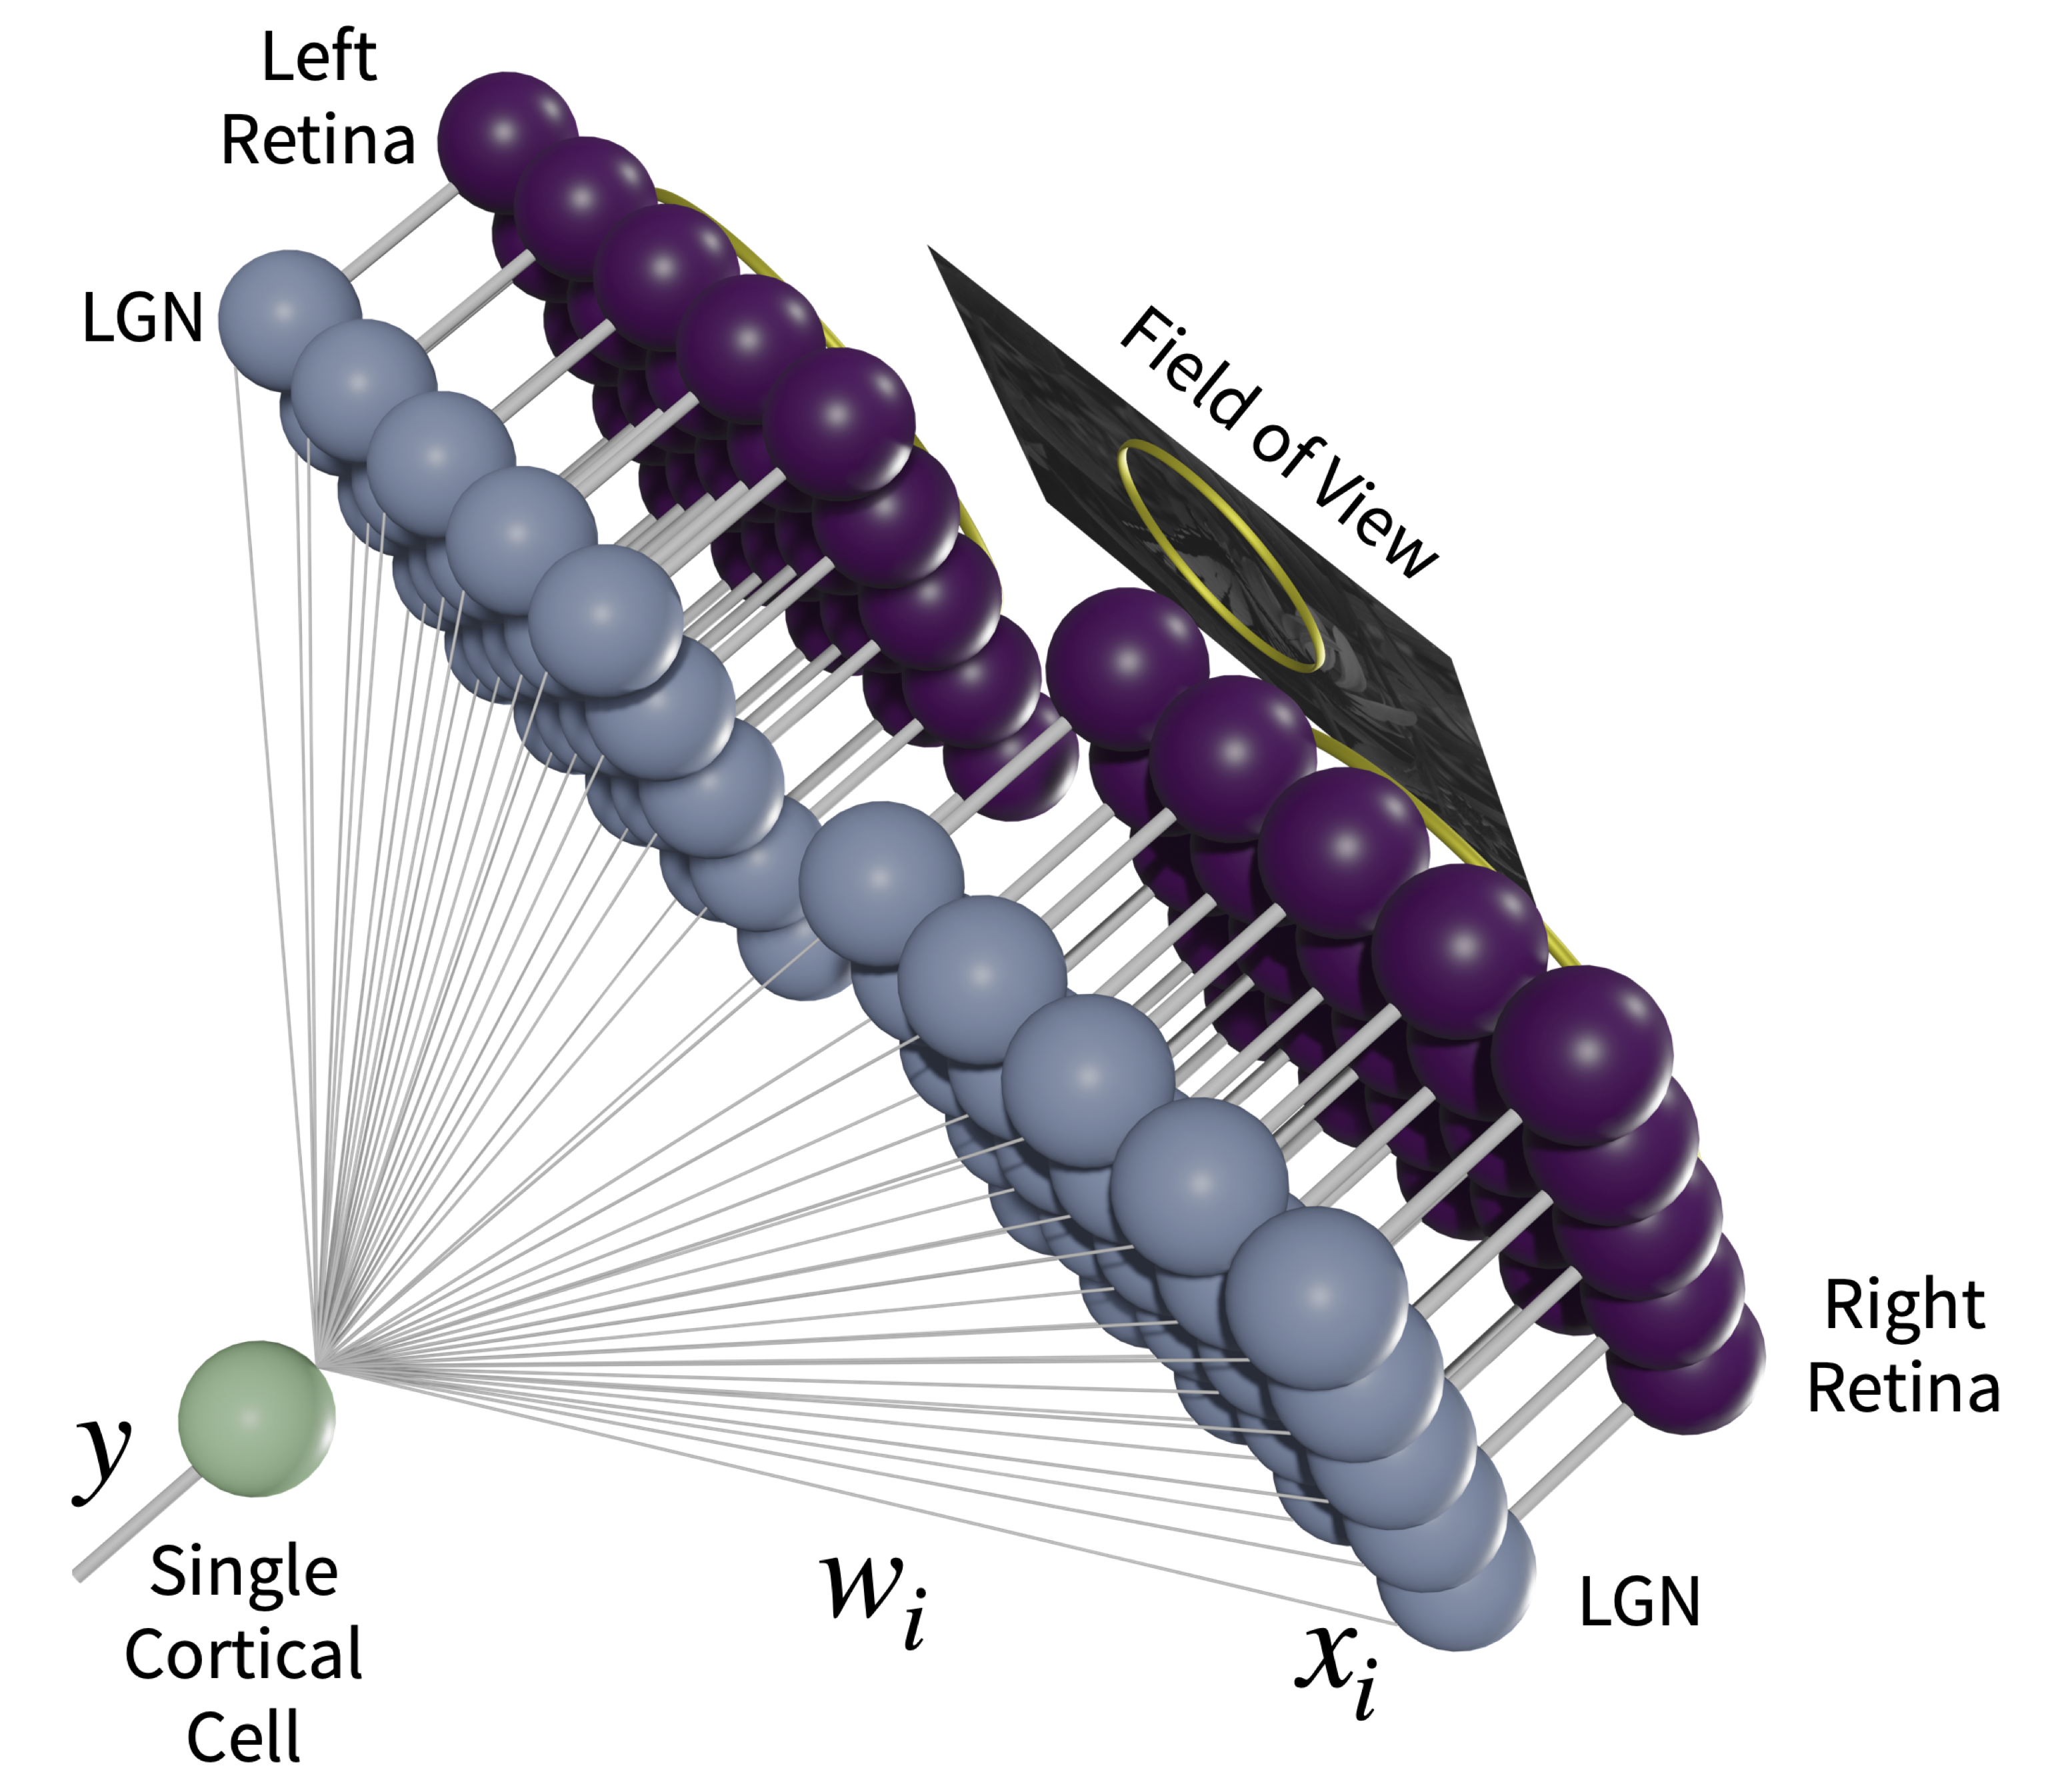
\includegraphics{/Users/bblais/Documents/Git/Amblyopia-Simulation/Manuscript/resources/arch.png}
\caption{Two-eye architecture.}\label{fig:arch}
}
\end{figure}

\begin{figure}
\hypertarget{fig:normal-inputs}{%
\centering
\includesvg{/Users/bblais/Documents/Git/Amblyopia-Simulation/Manuscript/resources/fig-normal_patches.svg}
\caption{A sample of 24 input patches from a normal visual environment
with jitter parameters \(\mu_c=0\) and \(\sigma_c=0\). The left- and
right-eye inputs are shown in pairs.}\label{fig:normal-inputs}
}
\end{figure}

\hypertarget{synaptic-modification-the-bcm-learning-rule}{%
\subsection{Synaptic Modification: The BCM Learning
Rule}\label{synaptic-modification-the-bcm-learning-rule}}

We use a single neuron and the parabolic form of the BCM(Bienenstock et
al., 1982; Brian S. Blais et al., 2008) learning rule for all of the
simulations, where the synaptic modification depends on the postsynaptic
activity, \(y\), in the following way for a single neuron

\[
y=\sigma\left(\sum_i x_i w_i \right)
\] \[
\frac{dw_i}{dt} = \eta y(y-\theta_M) x_i
\] \[
\frac{d\theta_M}{dt} = (y^2-\theta_M)/\tau
\]

where is \(x_i\) is the \(i\)th presynaptic input, \(w_i\) is the
\(i\)th synaptic weight, and \(y\) is the postsynaptic output activity.
The constant, \(\eta\), refers to the learning rate and the constant,
\(\tau\), is what we call the memory-constant and is related to the
speed of the sliding threshold. The transfer function,
\(\sigma(\cdot)\), places minimum and maximum responses given a set of
inputs and weights.

\begin{figure}
\hypertarget{fig:bcm-phi}{%
\centering
\includesvg{/Users/bblais/Documents/Git/Amblyopia-Simulation/Manuscript/resources/fig-bcm-phi.svg}
\caption{The BCM synaptic modification function. Units are
arbitrary.}\label{fig:bcm-phi}
}
\end{figure}

The results are extremely robust to values of \(\eta\) and \(\tau\) ,
which are generally chosen for practical, rather than theoretical,
considerations. Each of these constants is related to the time-step for
the simulations, but given the phenomenological nature of the BCM theory
it is beyond the scope of this paper to make detailed comparisons
between simulation time and real-time. Further, the fact that \(\tau\)
can be changed within a factor of 100 with no noticeable effect, the
experiments presented here cannot be used address the time-scales of the
molecular mechanisms underlying synaptic modification. Whenever we refer
to real-time units for a simulation, we approximate a single simulation
iteration as 1 iteration = 0.2 seconds(Brian S. Blais, 1998).

In the BCM learning rule, weights decrease if \(y\) is less than the
modification threshold,\(\theta_M\) , and increase if \(y\) is greater
than the modification threshold. To stabilize learning, the modification
threshold ``slides'' as a super-linear function of the output. The
output, \(y\) , is related to the product of the inputs and the weights
via a sigmoidal function, \(\sigma(\cdot)\), which places constraints on
the values of the output, keeping it in the range -1 and 50. The
interpretation of negative values is consistent with previous work(B. S.
Blais et al., 1998), where the activity values are measured relative to
spontaneous activity. Thus, negative values are interpreted as activity
below spontaneous. We continue this usage, in order to more easily
compare with previous simulations. The role of the spontaneous level for
the simulations in the natural image environment is discussed
elsewhere(B. S. Blais et al., 1998).

\hypertarget{simulation}{%
\subsection{Simulation}\label{simulation}}

The synaptic weights, and the modification threshold, are set to small
random initial values at the beginning of a simulation. At each
iteration, an input patch is generated as described above depending on
the procedure being simulated and then presented to the neuron. After
each input patch is presented, the weights are modified using the output
of the neuron, the input values and the current value of the
modification threshold. In an input environment composed of patches
taken from natural images, with equal patches presented to the left- and
right-eyes as shown in Figure \ref{fig:normal-inputs}, this process
orientation selective and fully binocular cells(B. S. Blais et al.,
1998). We then present test stimulus made from sine-gratings with 24
orientations, 20 spatial frequencies, and optimized over phase. Applying
any of the blur filters to the sine gratings does not quantitatively
change the result.

\begin{figure}
\hypertarget{fig:rf-theta-tuning-curve}{%
\centering
\includesvg{/Users/bblais/Documents/Git/Amblyopia-Simulation/Manuscript/resources/fig-rf-theta-tuning-curve.svg}
\caption{(A) Synaptic weights where black denotes weak weights and white
denotes strone weights. A clear preference for oriented stimuli can be
seen. (B) BCM modification threshold over time. The value converges to
nearly the same level for all neurons. (C) Responses to Oriented Stimuli
after training. Each neuron develops orientation selectivity to a range
of optimum angles.}\label{fig:rf-theta-tuning-curve}
}
\end{figure}

\hypertarget{models-of-development-of-amblyopia}{%
\subsection{Models of Development of
Amblyopia}\label{models-of-development-of-amblyopia}}

Amblyopia is a reduction of the best-corrected visual acuity (BCVA) with
an otherwise normal eye and has many causes(Wallace et al., 2018). Two
of the most common forms of amblyopia are strabismic and anisometropic
amblyiopia. Strabismic amblyopia occurs when the inputs from each eye do
not converge and the fixating eye becomes dominant over a non-fixating
eye. Refractive amblyopia occurs with untreated unilateral refractive
errors, one kind being anisometropic amblyopia where unequal refractive
power in each eye leads the retinal image from the amblyopic eye to be
blurred relative to the fellow eye. Both of these processes lead to
synaptic plasticity adjustments and interocular competition, enhancing
the initial deficit.

In this work we use a model of the amblyopic deficit caused by two
mechanisms. The first is a blurring of the amblyopic eye inputs,
representing refractive amblyopia. The second is eye-jitter,
representing one source of strabismic amblyopia(Charters and Ghasia,
2022). We have used the approximate values of \(\mu_c=7.5\) and
\(\sigma_c=2\) to represent significant strabismus -- nearly half of a
receptive field offset with a strong variation on the order of 25\% of
the RF size. We can explore these mechanisms independently and in
conjunction to see how they respond differentially to the various
treatments.

\hypertarget{refractive-amblyopia}{%
\subsubsection{Refractive amblyopia}\label{refractive-amblyopia}}

The amblyopic eye is presented with image patches that have been
\emph{blurred} with a normalized Gaussian filter applied to the images
with a specified width. The larger the width the blurrier the resulting
filtered image. Some examples are shown in Figure
\ref{fig:blurred-inputs}

\begin{figure}
\hypertarget{fig:blurred-inputs}{%
\centering
\includesvg{/Users/bblais/Documents/Git/Amblyopia-Simulation/Manuscript/resources/fig-blurred-inputs.svg}
\caption{A sample of 24 input patches from a refractive amblyopic
environment. The amblyopic (blurred) input is the square on the
left-hand side of each pair.}\label{fig:blurred-inputs}
}
\end{figure}

\hypertarget{strabismic-amblyopia}{%
\subsubsection{Strabismic amblyopia}\label{strabismic-amblyopia}}

Strabismic inputs are modeled by changing the center of the left- and
right-input patches in a systematic way, with a set mean offset
(\(\mu_c\)) and a standard deviation (\(\sigma_c\)) per input patch
generated. In this way we can model completely overlapping (\(\mu_c=0\))
inputs, completely non-overlapping (i.e.~extreme strabismus,
\(\mu_c>19\)), and any amount of overlap in between. Some examples are
shown in Figure \ref{fig:jitter-inputs} with the offset locations shown
in Figure \ref{fig:jitter-input-locations}.

\begin{figure}
\hypertarget{fig:jitter-inputs}{%
\centering
\includesvg{/Users/bblais/Documents/Git/Amblyopia-Simulation/Manuscript/resources/fig-jitter-inputs.svg}
\caption{A sample of 24 input patches from a strabismic visual
environment achieved through random jitter between the amblyopic (left)
eye and the fellow (right) eye.}\label{fig:jitter-inputs}
}
\end{figure}

\begin{figure}
\hypertarget{fig:jitter-input-locations}{%
\centering
\includesvg{/Users/bblais/Documents/Git/Amblyopia-Simulation/Manuscript/resources/fig-jitter-locations.svg}
\caption{Locations of the center of the left- and right-field of view
receptive fields, jittered randomly with set mean and standard
deviation. The average receptive fields are shown as gray
squares.}\label{fig:jitter-input-locations}
}
\end{figure}

\hypertarget{models-of-treatments-for-amblyopia}{%
\subsection{Models of Treatments for
Amblyopia}\label{models-of-treatments-for-amblyopia}}

\hypertarget{optical-fix}{%
\subsubsection{Optical Fix}\label{optical-fix}}

To model the fix to the refractive imbalance we follow the deficit
simulation described above with an input environment that is rebalanced.
Both eyes receiving nearly identical input patches
(\ref{fig:normal-inputs}) without any blur filter on the amblyopic eye
but with the same jitter and noise deviations as described above. This
process is a model of the application of refractive correction.

\hypertarget{patch-treatment}{%
\subsubsection{Patch treatment}\label{patch-treatment}}

The typical patch treatment is done by depriving the fellow-eye of input
with an eye-patch. In the model this is equivalent to presenting the
fellow-eye (taken to be the right-eye in the simulations) with random
noise instead of the natural image input. Competition between the left-
and right-channels drives the recovery, and is produced from the
difference between \emph{structured} input into the amblyopic-eye and
the \emph{unstructured} (i.e.~noise) input into the fellow eye. It is
not driven by a reduction in input activity. \ref{fig:patch-inputs}
shows sample simulation input patterns from the patched eye. Compare
this to \ref{fig:normal-inputs} to see that the simulated patch has far
less structure than the normal inputs.

\begin{figure}
\hypertarget{fig:patch-inputs}{%
\centering
\includesvg{/Users/bblais/Documents/Git/Amblyopia-Simulation/Manuscript/resources/fig-patch-inputs.svg}
\caption{A sample of 24 input patches from a patched visual environment.
Shown is the input to the amblyopic eye (left) which is the normal
visual environment and the input to the fellow eye (right) which
consists of random noise.}\label{fig:patch-inputs}
}
\end{figure}

\hypertarget{contrast-modification}{%
\subsubsection{Contrast modification}\label{contrast-modification}}

A binocular approach to treatment can be produced with contrast
reduction of the non-deprived channel relative to the deprived channel.
Experimentally this can be accomplished with VR headsets(Xiao et al.,
2020). In the model we implement this by down-scaling the fellow-eye
channel with a simple scalar multiplier applied to each pixel. The
contrast difference sets up competition between the two channels with
the advantage given to the amblyopic-eye channel.

\begin{figure}
\hypertarget{fig:contrast-modified-inputs}{%
\centering
\includesvg{/Users/bblais/Documents/Git/Amblyopia-Simulation/Manuscript/resources/fig-contrast-modified-inputs.svg}
\caption{A sample of 24 input patches from a contrast modified visual
environment. Shown is the input to the amblyopic eye (left) which is the
normal visual environment and the input to the fellow eye (right) which
is the same input but with contrast
reduced.}\label{fig:contrast-modified-inputs}
}
\end{figure}

\hypertarget{atropine-treatment}{%
\subsubsection{Atropine treatment}\label{atropine-treatment}}

In the atropine treatment for amblyopia(Glaser et al., 2002), eye-drops
of atropine are applied to the fellow-eye resulting in blurred vision in
that eye. Here we use the same blurred filter used to obtain the deficit
(possibly with a different width) applied to the fellow eye (Figure
\ref{fig:atropine-inputs}). The difference in sharpness between the
fellow-eye inputs and the amblyopic-eye inputs sets up competition
between the two channels with the advantage given to the amblyopic-eye.

\begin{figure}
\hypertarget{fig:atropine-inputs}{%
\centering
\includesvg{/Users/bblais/Documents/Git/Amblyopia-Simulation/Manuscript/resources/fig-atropine-inputs.svg}
\caption{A sample of 24 input patches from a simulated atropine
treatment environment. Shown is the input to the amblyopic eye (left)
which is the normal visual environment and the input to the fellow eye
(right) which is the same input but blurred with a Gaussian
filter.}\label{fig:atropine-inputs}
}
\end{figure}

\hypertarget{dichoptic-masks}{%
\subsubsection{Dichoptic Masks}\label{dichoptic-masks}}

On top of the contrast modification, we can include the application of
the dichoptic mask. In this method, each eye receives a version of the
input images filtered through independent masks in each channel,
resulting in a mostly-independent pattern in each channel. It has been
observed that contrast modification combined with dichoptic masks can be
an effective treatment for amblyopiaXiao et al. (2022). The motivation
behind the application of the mask filter is that the neural system must
use both channels to reconstruct the full image and thus may lead to
enhanced recovery.

The dichoptic masks are constructed with the following procedure. A
blank image (i.e.~all zeros) is made to which is added 15 randomly sized
circles with values equal to 1 (Figure \ref{fig:dichopic_blob} A). These
images are then smoothed with a Gaussian filter of a given width, \(f\)
(Figure \ref{fig:dichopic_blob} B). This width is a parameter we can
vary to change the overlap between the left- and right-eye images. A
high value of \(f\) compared with the size of the receptive field,
e.g.~\(f=90\), yields a high overlap between the patterns in the
amblyopic- and fellow-eye inputs (Figure
\ref{fig:dichopic_filter_size}). Likewise, a small value of \(f\),
e.g.~\(f=10\), the eye inputs are nearly independent -- the patterned
activity falling mostly on one of the eyes and not much to both.
Finally, the smoothed images are scaled to have values from a minimum of
0 to a maximum of 1. This image-mask we will call \(A\), and is the
left-eye mask whereas the right-eye mask, \(F\), is the inverse of the
left-eye mask, \(F\equiv 1-A\). The mask is applied to an image by
multiplying the left- and right-eye images by the left- and right-eye
masks, respectively, resulting in a pair of images which have no overlap
at the peaks of each mask, and nearly equal overlap in the areas of the
images where the masks are near 0.5 (Figure
\ref{fig:dichopic_filter_image}).

\begin{figure}
\hypertarget{fig:dichopic_blob}{%
\centering
\includesvg{/Users/bblais/Documents/Git/Amblyopia-Simulation/Manuscript/resources/blob_convolution_example_fsig_20.svg}
\caption{The dichoptic masks are produced by taking random circular
blobs (A), convolving them a Gaussian filter of a specified size (B),
resulting in the circular blobs blending into the background smoothly at
the edges on the scale of the filter (C)}\label{fig:dichopic_blob}
}
\end{figure}

\begin{figure}
\hypertarget{fig:dichopic_filter_size}{%
\centering
\includesvg{/Users/bblais/Documents/Git/Amblyopia-Simulation/Manuscript/resources/mask_filter_examples_fsigs.svg}
\caption{The dichoptic masks for several different filter sizes. The
larger the filter, the larger the overlap in the patterns presented to
the two eyes. For a very sharp mask (upper left) patterns are nearly all
to either the left or the right eye. For a wide mask (lower right) most
patterns are presented to both eyes.}\label{fig:dichopic_filter_size}
}
\end{figure}

\begin{figure}
\hypertarget{fig:dichopic_filter_image}{%
\centering
\includesvg{/Users/bblais/Documents/Git/Amblyopia-Simulation/Manuscript/resources/mask_filter_example_fsig_20.svg}
\caption{An example of a dichoptic mask, \(\sigma_f = 20\), applied to
one of the images. The mask (A) shows how much of the input goes to each
of the left and right channels. The resulting left- and right-images (B
and C, respectively) show the results of the partial independence of the
two channels. One can see areas where there is some overlap as well as
areas where the pattern is only present in one of the eyes due to the
application of the mask.}\label{fig:dichopic_filter_image}
}
\end{figure}

\hypertarget{quantifying-responses}{%
\subsection{Quantifying responses}\label{quantifying-responses}}

\hypertarget{ocular-dominance-index}{%
\subsubsection{Ocular Dominance Index}\label{ocular-dominance-index}}

Simulations are ended when selectivity has been achieved and the
responses are stable. From the maximal responses of each eye,
\(R_{\text{left}}\) and \(R_{\text{right}}\), individually, we can
calculate the ocular dominance index as \[
\text{ODI} \equiv \frac{R_{\text{right}}-R_{\text{left}}}{R_{\text{right}}+R_{\text{left}}}
\] The ocular dominance index (ODI) has a value of
\(\text{ODI} \approx 1\) when stimulus to the right-eye (typically the
fellow eye in the simulations, by convention) yields a maximum neuronal
response with little or no contribution from the left-eye. Likewise, an
ocular dominance index (ODI) has a value of \(\text{ODI} \approx -1\)
when stimulus to the left-eye (typically the amblyopic eye, by
convention) yields a maximum neuronal response with little or no
contribution from the right-eye. A value of \(\text{ODI} \approx 0\)
represents a purely binocular cell, responding equally to stimulus in
either eye.

\hypertarget{results}{%
\section{Results}\label{results}}

\hypertarget{refractory-and-strabismic-amblyopia}{%
\subsection{Refractory and Strabismic
Amblyopia}\label{refractory-and-strabismic-amblyopia}}

Figure \ref{fig:deficit} shows the production of a deficit effect using
both refractory blurring and inter-eye jitter. The refractory blur has a
much larger effect, with larger blur resulting in a more pronounced
deficit. For the sake of convenience, we use a blur=4 for the rest of
the simulations because it gives a robust deficit effect without being
overwhelming.

\begin{figure}
\hypertarget{fig:deficit}{%
\centering
\includesvg{/Users/bblais/Documents/Git/Amblyopia-Simulation/Manuscript/resources/fig-deficit-response-ODI-blur.svg}
\caption{Deficit maximum response for the amblyopic- and fellow-input
channels (A) and the resulting ODI (B) as a function of the deficit blur
size (in pixels) with several combinations of the jitter offset mean
(\(\mu_c\)) standard deviation (\(\sigma_c\)). Interestingly, the jitter
does very little other than make the variation
higher.}\label{fig:deficit}
}
\end{figure}

\hypertarget{treatments}{%
\subsection{Treatments}\label{treatments}}

\hypertarget{optical-fix-1}{%
\subsubsection{Optical Fix}\label{optical-fix-1}}

Shown in Figure \ref{fig:fix-response-ODI-blur} are the results for the
optical fix as a function of the open-eye noise. For larger open-eye
noise, the recovery rate (Figure \ref{fig:fix-response-ODI-blur} C)
increases. Changing jitter increases the variability and seems to
increase the effectiveness of the treatment, at least for low-noise, but
the results are not statistically significant.

\begin{figure}
\hypertarget{fig:fix-response-ODI-blur}{%
\centering
\includesvg{/Users/bblais/Documents/Git/Amblyopia-Simulation/Manuscript/resources/fig-fix-response-ODI-blur.svg}
\caption{Optical fix treatment (A) maximum response for the amblyopic-
and fellow-input channels, (B) the resulting ODI and (C) the recovery
rate (i.e.~ODI shift per time). Each is shown as a function of the
open-eye noise with several combinations of the jitter offset mean
(\(\mu_c\)) standard deviation
(\(\sigma_c\)).}\label{fig:fix-response-ODI-blur}
}
\end{figure}

\hypertarget{patch-treatment-1}{%
\subsubsection{Patch Treatment}\label{patch-treatment-1}}

Shown in Figure \ref{fig:patch-response-ODI-blur} are the results for
the patch treatment as a function of the closed-eye noise. For larger
closed-eye noise, the recovery rate (Figure
\ref{fig:patch-response-ODI-blur} C) increases -- up to a high level of
noise, where it tapers off. Changing jitter increases the variability
and seems to increase the effectiveness of the treatment -- especially
for the mean value of the jitter. Above a noise level of 0.5 the
variability becomes so large that no further recovery can be seen.

It is surprising that we don't get a reverse amblyopia effect for large
noise, but it may be masked by the increased variability.

\begin{figure}
\hypertarget{fig:patch-response-ODI-blur}{%
\centering
\includesvg{/Users/bblais/Documents/Git/Amblyopia-Simulation/Manuscript/resources/fig-patch-response-ODI-blur.svg}
\caption{Patch treatment (A) maximum response for the amblyopic- and
fellow-input channels, (B) the resulting ODI and (C) the recovery rate
(i.e.~ODI shift per time). Each is shown as a function of the open-eye
noise with several combinations of the jitter offset mean (\(\mu_c\))
standard deviation (\(\sigma_c\)).}\label{fig:patch-response-ODI-blur}
}
\end{figure}

\hypertarget{atropine-treatment-1}{%
\subsubsection{Atropine Treatment}\label{atropine-treatment-1}}

Shown in Figure \ref{fig:atropine-response-ODI-blur} are the results for
the atropine treatment as a function of the blur size. For larger blur
size, the recovery rate (Figure \ref{fig:patch-response-ODI-blur} C)
increases and saturates at a point lower than that for patch treatment.
As for the other treatments, changing jitter increases the variability
but has little other effect.

\begin{figure}
\hypertarget{fig:atropine-response-ODI-blur}{%
\centering
\includesvg{/Users/bblais/Documents/Git/Amblyopia-Simulation/Manuscript/resources/fig-atropine-response-ODI-blur.svg}
\caption{Atropine treatment (A) maximum response for the amblyopic- and
fellow-input channels, (B) the resulting ODI and (C) the recovery rate
(i.e.~ODI shift per time). Each is shown as a function of the open-eye
noise with several combinations of the jitter offset mean (\(\mu_c\))
standard deviation
(\(\sigma_c\)).}\label{fig:atropine-response-ODI-blur}
}
\end{figure}

\hypertarget{contrast-and-mask}{%
\subsection{Contrast and Mask}\label{contrast-and-mask}}

\begin{figure}
\hypertarget{fig:mask-response-ODI-contrast-mu0-sigma0}{%
\centering
\includesvg{/Users/bblais/Documents/Git/Amblyopia-Simulation/Manuscript/resources/fig-mask-response-ODI-contrast-mu0-sigma0.svg}
\caption{Dichoptic mask treatment (A) maximum response for the
amblyopic- and fellow-input channels, (B) the resulting ODI and (C) the
recovery rate (i.e.~ODI shift per time) for the case of jitter offset
mean \(\mu_c=0\) and standard deviation \(\sigma_c=0\). This is the no
eye-jitter case. Each quantity is shown as a function of the contrast
applied to the fellow eye. Contrast=1 means no contrast difference
between the fellow- and amblyopic-eye inputs. Contrast=0 means that the
fellow eye is completely silent, except for possible added noise. Shown
in black is the no-mask situation. The size of the mask moves from a
sharp mask with little input overlap, \(\sigma_f=10\), to a fuzzy mask
with a large amount of input overlap,
\(\sigma_f=90\).}\label{fig:mask-response-ODI-contrast-mu0-sigma0}
}
\end{figure}

Figure \ref{fig:mask-response-ODI-contrast-mu0-sigma0} shows the effect
of contrast and dichoptic masks for the case of no eye-jitter while
Figure \ref{fig:mask-response-ODI-contrast-mu75-sigma2} shows the same
for a large eye-jitter. The mask enhances the rate of recovery for small
contrasts (contrast\textless0.4), and doesn't affect the cases for high
contrast where there is no recovery. These high-contrast cases have the
fellow eye dominant.

\begin{figure}
\hypertarget{fig:mask-response-ODI-contrast-mu75-sigma2}{%
\centering
\includesvg{/Users/bblais/Documents/Git/Amblyopia-Simulation/Manuscript/resources/fig-mask-response-ODI-contrast-mu75-sigma2.svg}
\caption{Dichoptic mask treatment (A) maximum response for the
amblyopic- and fellow-input channels, (B) the resulting ODI and (C) the
recovery rate (i.e.~ODI shift per time) for the case of jitter offset
mean \(\mu_c=0\) and standard deviation \(\sigma_c=0\). This is the no
eye-jitter case. Each quantity is shown as a function of the contrast
applied to the fellow eye. Contrast=1 means no contrast difference
between the fellow- and amblyopic-eye inputs. Contrast=0 means that the
fellow eye is completely silent, except for possible added noise. Shown
in black is the no-mask situation. The size of the mask moves from a
sharp mask with little input overlap, \(\sigma_f=10\), to a fuzzy mask
with a large amount of input overlap,
\(\sigma_f=90\).}\label{fig:mask-response-ODI-contrast-mu75-sigma2}
}
\end{figure}

Both Figure \ref{fig:mask-response-ODI-contrast-mu0-sigma0} and Figure
\ref{fig:mask-response-ODI-contrast-mu75-sigma2} show a marked reverse
amblyopia effect in the time-frame of the simulation -- because the
recovery rate is so high. It seems to be tempered somewhat with a
sharper mask, but more simulations need to be run to see if the effect
is statistically significant. This suggests that, in addition to
increasing the contrast of the fellow eye, one could modify the mask to
reduce the chance of reverse amblyopia.

\hypertarget{conclusions-and-discussion}{%
\section{Conclusions and Discussion}\label{conclusions-and-discussion}}

While the results of this work are promising, there are a number of
limitations. This model is a single-neuron model which means it doesn't
take into account any network effects, such as the balance of excitatory
and inhibitory influences. It also is an early-vision model, so it does
not include any object recognition, higher-order vision processes or
memory processes that may be involved with amblyopia. We measure ocular
dominance for convenience because spatial frequency, which would be a
more natural quantity to use for amblyopia, is to noisy for a model with
19x19 input patches. Finally, this is not a biophysical model, so neuron
spike-effects are not covered.

However, the model does allow one to run many different scenarios with
as few assumptions as possible. It can capture the dynamics of the
learning in the visual system in these scenarios, and allows us to
explore the benefits and drawbacks of different treatment paradigms.

Given that both the contrast of the fellow eye and the dichoptic mask
influence the rate of recovery, one could modify the mask or the
contrast to reduce the chance of reverse amblyopia. One would want
frequent measurements of the inter-eye imbalance to recognize when such
a change is warranted.

\hypertarget{some-lingering-questions}{%
\subsubsection{Some lingering
questions}\label{some-lingering-questions}}

Here are just a couple of things I noticed, that I need to look into to
see if there are any issues.

\begin{itemize}
\tightlist
\item[$\square$]
  I would have expected a reverse amblyopia effect with the patch
  treatment, but I don't see that. It might be washed out in the
  variation at high noise level, but I want to be sure
\item[$\square$]
  I would have expected that in the dichoptic treatment, that the case
  of contrast=1 with no mask would be identical to the optical fix at an
  open-eye noise level of 0.1. I don't see that, so I am not sure what
  the difference is
\item[$\square$]
  I think it would be useful to run a couple of these cases for more
  systematic changes in the jitter mean and standard deviation. There
  wasn't much of an effect, but it is there in places and it would be
  easier to communicate this with a few examples
\end{itemize}

\hypertarget{references}{%
\section*{References}\label{references}}
\addcontentsline{toc}{section}{References}

\hypertarget{refs}{}
\begin{CSLReferences}{1}{0}
\leavevmode\vadjust pre{\hypertarget{ref-BCM82}{}}%
Bienenstock, E. L., Cooper, L. N., and Munro, P. W. (1982). Theory for
the development of neuron selectivity: Orientation specificity and
binocular interaction in visual cortex. \emph{Journal of Neuroscience},
\emph{2}, 32--48.

\leavevmode\vadjust pre{\hypertarget{ref-birch2013amblyopia}{}}%
Birch, E. E. (2013). Amblyopia and binocular vision. \emph{Progress in
Retinal and Eye Research}, \emph{33}, 67--84.

\leavevmode\vadjust pre{\hypertarget{ref-phd:Blais98}{}}%
Blais, Brian S. (1998, May). \emph{The role of the environment in
synaptic plasticity:\\
towards an understanding of learning and memory} (PhD thesis). Brown
University, Institute for Brain; Neural Systems; Dr. Leon N Cooper,
Thesis Supervisor.

\leavevmode\vadjust pre{\hypertarget{ref-Blais:2008kx}{}}%
Blais, Brian S., Frenkel, M. Y., Kuindersma, S. R., Muhammad, R.,
Shouval, H. Z., Cooper, L. N., and Bear, M. F. (2008).
\href{https://doi.org/10.1152/jn.90411.2008}{Recovery from monocular
deprivation using binocular deprivation}. \emph{J Neurophysiol},
\emph{100}(4), 2217--24.

\leavevmode\vadjust pre{\hypertarget{ref-BlaisEtAl98}{}}%
Blais, B. S., Intrator, N., Shouval, H., and Cooper, L. N. (1998).
Receptive field formation in natural scene environments: Comparison of
single cell learning rules. \emph{Neural Computation}, \emph{10}(7),
1797--1813.

\leavevmode\vadjust pre{\hypertarget{ref-carandini2012normalization}{}}%
Carandini, M., and Heeger, D. J. (2012). Normalization as a canonical
neural computation. \emph{Nature Reviews Neuroscience}, \emph{13}(1),
51--62.

\leavevmode\vadjust pre{\hypertarget{ref-Charters:2022aa}{}}%
Charters, L., and Ghasia, F. (2022). Unraveling the mysteries of
amblyopia and fixation eye movements. \emph{Ophthalmology Times},
\emph{47}(4).

\leavevmode\vadjust pre{\hypertarget{ref-DeAngelis:1995aa}{}}%
DeAngelis, G. C., Ohzawa, I., and Freeman, R. D. (1995). Receptive-field
dynamics in the central visual pathways. \emph{Trends in Neurosciences},
\emph{18}(10), 451--458.

\leavevmode\vadjust pre{\hypertarget{ref-Gao_2018}{}}%
Gao, T. Y., Guo, C. X., Babu, R. J., Black, J. M., Bobier, W. R.,
Chakraborty, A., \ldots{} al., et. (2018).
\href{https://doi.org/10.1001/jamaophthalmol.2017.6090}{Effectiveness of
a binocular video game vs placebo video game for improving visual
functions in older children, teenagers, and adults with amblyopia}.
\emph{JAMA Ophthalmology}, \emph{136}(2), 172.

\leavevmode\vadjust pre{\hypertarget{ref-glaser2002randomized}{}}%
Glaser, S. R., Matazinski, A. M., Sclar, D. M., Sala, N. A., Vroman, C.
M., Tanner, C. E., et al.others. (2002). A randomized trial of atropine
vs patching for treatment of moderate amblyopia in children.
\emph{Archives of Ophthalmology}, \emph{120}(3), 268--278.

\leavevmode\vadjust pre{\hypertarget{ref-hess2015amblyopia}{}}%
Hess, R. F., and Thompson, B. (2015). Amblyopia and the binocular
approach to its therapy. \emph{Vision Research}, \emph{114}, 4--16.

\leavevmode\vadjust pre{\hypertarget{ref-Holmes_2016}{}}%
Holmes, Jonathan M., Manh, V. M., Lazar, E. L., Beck, R. W., Birch, E.
E., Kraker, R. T., \ldots{} al., et. (2016a).
\href{https://doi.org/10.1001/jamaophthalmol.2016.4262}{Effect of a
binocular iPad game vs part-time patching in children aged 5 to 12 years
with amblyopia}. \emph{JAMA Ophthalmology}, \emph{134}(12), 1391.

\leavevmode\vadjust pre{\hypertarget{ref-holmes2016randomized}{}}%
Holmes, Jonathan M., Manh, V. M., Lazar, E. L., Beck, R. W., Birch, E.
E., Kraker, R. T., et al.others. (2016b). A randomized trial of a
binocular iPad game versus part-time patching in children 5 to 12 years
of age with amblyopia. \emph{JAMA Ophthalmology}, \emph{134}(12), 1391.

\leavevmode\vadjust pre{\hypertarget{ref-Kelly_2016}{}}%
Kelly, K. R., Jost, R. M., Dao, L., Beauchamp, C. L., Leffler, J. N.,
and Birch, E. E. (2016).
\href{https://doi.org/10.1001/jamaophthalmol.2016.4224}{Binocular iPad
game vs patching for treatment of amblyopia in children}. \emph{JAMA
Ophthalmology}, \emph{134}(12), 1402.

\leavevmode\vadjust pre{\hypertarget{ref-Li:2015aa}{}}%
Li, S. L., Reynaud, A., Hess, R. F., Wang, Y.-Z., Jost, R. M., Morale,
S. E., \ldots{} Birch, E. E. (2015).
\href{https://doi.org/10.1016/j.jaapos.2015.08.003}{Dichoptic movie
viewing treats childhood amblyopia}. \emph{J AAPOS}, \emph{19}(5),
401--5.

\leavevmode\vadjust pre{\hypertarget{ref-Ruderman:1994aa}{}}%
Ruderman, D. L., and Bialek, W. (1994). Statistics of natural images:
Scaling in the woods. \emph{Physical Review Letters}, \emph{73}(6), 814.

\leavevmode\vadjust pre{\hypertarget{ref-wallace2018amblyopia}{}}%
Wallace, D. K., Repka, M. X., Lee, K. A., Melia, M., Christiansen, S.
P., Morse, C. L., and Sprunger, D. T. (2018). Amblyopia preferred
practice pattern{\textregistered}. \emph{Ophthalmology}, \emph{125}(1),
P105--P142.

\leavevmode\vadjust pre{\hypertarget{ref-xiao2022randomized}{}}%
Xiao, S., Angjeli, E., Wu, H. C., Gaier, E. D., Gomez, S., Travers, D.
A., et al.others. (2022). Randomized controlled trial of a dichoptic
digital therapeutic for amblyopia. \emph{Ophthalmology}, \emph{129}(1),
77--85.

\leavevmode\vadjust pre{\hypertarget{ref-xiao2020improved}{}}%
Xiao, S., Gaier, E. D., Mazow, M. L., Stout, A. U., Travers, D. A.,
Angjeli, E., \ldots{} Hunter, D. G. (2020). Improved adherence and
treatment outcomes with an engaging, personalized digital therapeutic in
amblyopia. \emph{Scientific Reports}, \emph{10}(1), 1--8.

\leavevmode\vadjust pre{\hypertarget{ref-de2007current}{}}%
Zárate, B. R. de, and Tejedor, J. (2007). Current concepts in the
management of amblyopia. \emph{Clinical Ophthalmology (Auckland, NZ)},
\emph{1}(4), 403.

\end{CSLReferences}

\end{document}
